\subsection{Введение в метод конечных элементов}

Метод конечных элементов(МКЭ) — это численная процедура решения задач,
сформулированных в виде дифференциального уравнения или вариационного 
принципа.[2]
МКЭ возник как универсальный метод для решения дифференциальных уравнений. 
Метод приобрел большую популярность, так как он позволяет анализировать и
решать широкий спектр задач.


Метод конечных элементов отличается от классических
методов Ритца и Галеркина тем, что аппроксимирующая функция является
линейной комбинацией непрерывных кусочно-гладких финитных функций.
Финитные функции отличны от нуля только в заданном интервале.
В МКЭ под такими интервалами подразумеваются конечные элементы, на
которые разбивается область $\Omega$. 


Термин метод конечных элементов, в действительности, определяет
широкий спектр вычислительных технологий в соответствии с некоторы-
ми общими свойствами. Процесс конечно-элементного анализа включает
определенную последовательность шагов. Перечислим эти шаги.

1. Дискретизация области: построение сетки, задание свойств (материала)
элементов. Область, на которой решается задача, аппроксимируется
(покрывается) непересекающимися подобластями простого типа, которые
называются конечными элементами (КЭ)(Рисунок 1).

\renewcommand{\figurename}{Рисунок}
\begin{figure}[H]
      \centering
      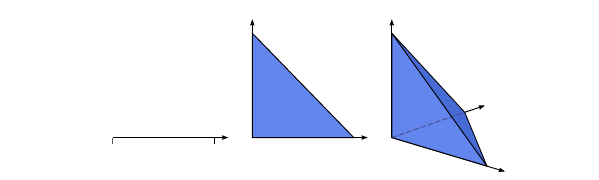
\includegraphics[width=0.8\textwidth]{./pics/random-cells.png}\\
      \centering\caption{Пример конечно-элементных подобластей для пространств размерности n = 1,2,3}
\end{figure}
Множество элементов, на которые разбита область, называется конечно-элементной сеткой. Вершины КЭ
называются узлами. Узлы предназначены для описания геометрии элемента
и для задания компонент решения (неизвестная величина задается в узлах).
Узлы могут быть внешними и внутренними. Внешние узлы лежат на границе КЭ и используются для соединения элементов друг с другом. Так же элементы могут располагаться между угловыми узлами.
КЭ может иметь и внутренние узлы, такие элементы обеспечивают более точное описание
искомых функций. 

Компоненты решения в узле называются степенями
свободы. В зависимости от рассматриваемых задач число степеней свободы
в узле различно. Например, если рассматривается задача теплопроводности,
в каждой точке ищется одно значение температуры — одна степень
свободы. А если рассматривается двумерная задача упругости относитель
но неизвестных перемещений, то число компонент будет равно двум, так
как перемещение величина векторная $u = (ux, uy)$. В качестве степеней
свободы могут фигурировать как узловые значения неизвестной функции,
так и ее производные по пространственным координатам в узлах. Кроме 
того необходимо задать свойства материала, из которого изготовлена
конструкция или КЭ. Например, для изотропных тел при решении задач
теории упругости необходимо знать такие константы, как модуль Юнга
и коэффициент Пуассона материала, при решении задачи теплопроводно-
сти — коэффициент теплопроводности

Как только область разбита на соответствующие подобласти, на каждой такой подобласти можно 
определить функциональное пространство $V$ и использовать каждое $V$ для определения глобального
функционального пространства $V_h$. Подобласть $T$ вместе с определенным на ней функциональным пространством $V$ называется конечным элементом. Более строгое определение:

\begin{itemize}
    \item Подобласть $T$ - замкнута, с кусочно-гладкой границей
    \item Область $V(T)$ - конечное функциональное пространство на $T$
\end{itemize}

2. Формирование СЛАУ с учетом вкладов от элементов и узлов, введе-
ние граничных условий в систему уравнений. Например, если задача реша-
ется с помощью метода Галеркина (метода взвешенных невязок) форми-
руются интегралы от произведения невязки на весовые функции, которые
затем приравниваются к нулю. Если решается задача в вариационной по-
становке с помощью метода Ритца минимизации функционала, то СЛАУ
получается после приравнивания к нулю производных функционала

3. Формирование СЛАУ с учетом вкладов от элементов и узлов, введение 
граничных условий в систему уравнений. 

4. Решение полученной системы уравнений.
Точное решение дифференциального уравнения при подстановке в это
дифференциальное уравнение обращает его в тождество в каждой точке.
Решение МКЭ предполагает, что приближенное решение $u_h$ будет удовлетворять
дифференциальному уравнению в узлах сетки $u_h(x_i, t) = u(x_i, t) = u_i^t$.

5. Определение расчетных величин в элементах. Этими величинами
обычно являются производные от неизвестной функции (например, дефор-
мации, напряжения, тепловые потоки, скорости).

Точное решение дифференциального уравнения при подстановке в это
дифференциальное уравнение обращает его в тождество в каждой точке.
Решение МКЭ предполагает, что приближенное решение $\overline{u}$ будет удовле-
творять дифференциальному уравнению в узлах сетки $\overline{u}(x_i) = u(x_i) = u_i$
